% !TeX spellcheck = id_ID
\documentclass[a4paper,12pt]{article}
\usepackage[bahasa]{babel}
\usepackage{graphicx}
\usepackage{multirow}
\usepackage{enumitem}
\usepackage[T1]{fontenc}
\usepackage{inconsolata}
\usepackage{lipsum}
\usepackage{xcolor}
\usepackage{caption}

\graphicspath{ {./img/} }
\begin{document}
\title{ {\Large Laporan Praktikum}\\ Jaringan Komputer \\{\Large Pertemuan 13}}

\author{Aldzikri Dwijayanto Prathama 
	\\195410189
	\\Teknik Informatika}
\makeatletter
\begin{titlepage}
	\begin{center}
		{\huge \bfseries \@title }\\[14ex]
		
\includegraphics[scale=.8]{logo}\\[4ex]
		{\large \@author}\\[19ex]
		{\large \bfseries {SEKOLAH TINGGI MANAJEMEN INFORMATIKA DAN KOMPUTER
				AKAKOM YOGYAKARTA}}
	\end{center}


\end{titlepage}
\makeatother
\newpage
\tableofcontents
\newpage

\section{Tujuan}
\paragraph{}
Mahasiswa mampu melakukan konfigurasi pada Router untuk memblok akses internet
menggunakan Firewall.

\section{Dasar Teori}
\paragraph{}
\textit{Firewall} merupakan sebuah program perangkat lunak yang merupakan sistem
keamanan untuk mengelola dan memantau lalu lintas data yang keluar-masuk berdasarkan
aturan keamanan (\textit{security rules}) yang telah ditentukan. Firewall berfungsi mencegah
akses yang tidak diinginkan dari atau ke dalam jaringan atau server.
\paragraph{}
Jadi, \textit{firewall} adalah alat yang dapat digunakan untuk meningkatkan keamanan
komputer yang terhubung ke jaringan, seperti LAN atau Internet. \textit{Firewall} juga merupakan
bagian integral dari kerangka kerja keamanan komprehensif untuk jaringan yang
digunakan. \textit{Firewall} mampu menjamin keamanan melalui aktvitasi kontrol granular atas
jenis fungsi. \textit{Firewall} juga akan melangsungkan proses sistem yang memiliki akses ke
sumber daya jaringan.
Manfaat Firewall\\
\begin{itemize}
    \item \textbf{Melindungi komputer dari akses jarak jauh tidak sah.} Salah satu hal terburuk
    yang dapat terjadi pada perangkat jaringan adalah jika seseorang mencoba
    mengambil kendali dari jarak jauh, seperti mouse bergerak sendiri di monitor karena
    ulah hacker . Dengan melakukan konfigurasi yang benar pada firewall (dan OS
    modern), akses desktop jarak jauh dapat dinonaktifkan.
    \item \textbf{Dapat memblokir pesan yang menautkan ke konten yang tidak diinginkan.}
    Internet memiliki banyak kode buruk yang melintasi dunia maya, menunggu untuk
    menerkam PC yang tidak terlindungi. Firewall dapat mencegah hal ini terjadi.
    \item \textbf{Menjadikan kegiatan online lebih aman.} Setiap upaya yang dilakukan hacker
    untuk masuk ke dalam sistem akan diblokir.
\end{itemize}

\section{Praktik}
\begin{enumerate}[label=\textbf{\arabic*.}]
    \item \textbf{Instalasi Jaringan\\}
        \begin{itemize}
            \item Hubungkan jaringan kabel UTP dari laboratorium ke Ether 1.
            \item Hubungkan Ether 2 dengan PC1.
            \item Hubungkan Ether 5 dengan Swith (Port 1).
            \item Hubungkan Switch (Port 3) dengan PC2.
            \item Hubungkan Switch (Port 4) dengan PC3.
        \end{itemize}

    \item \textbf{Menghapus Konfigurasi Mikrotik\\}
        \begin{center}
            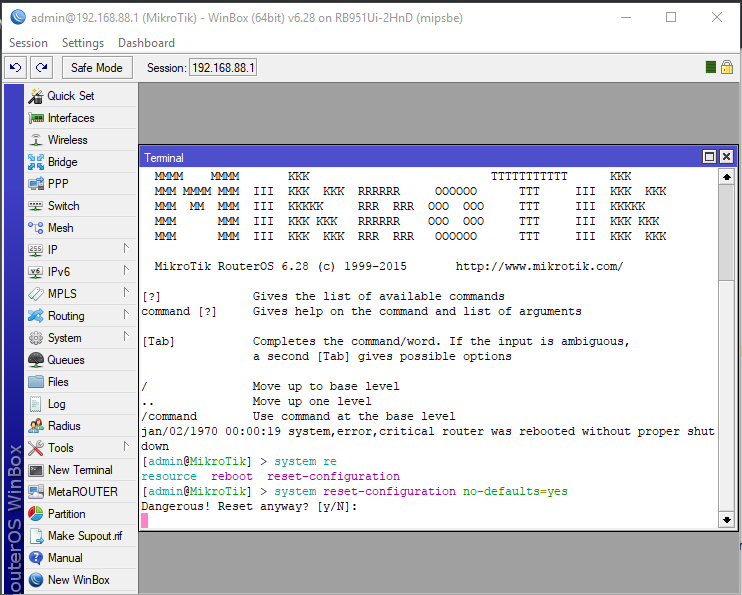
\includegraphics[width = 0.8\linewidth]{image1.png}
        \end{center}
        \begin{itemize}
            \item Login ke Mikrotik menggunakan WinBox.
            \item Klik menu New Terminal
            \item Pada prompt command line berikan perintah: \textcolor{red}{\texttt{/system reset-configuration no-default=yes}}
            \item Perintah ini menghapus semua konfigurasi router dan menetapkannya ke default untuk nama login dan kata sandi ('admin' dan tidak ada kata sandi), alamat IP dan konfigurasi lainnya akan dihapus, dan antarmuka akan menjadi dinonaktifkan.
            \item Tekan Enter, maka akan muncul pertanyaan, untuk konfirmasi apakah akan dilakukan Reset, masukkan y(yes), maka Mikrotik akan booting dan konfigurasinya telah dihapus semua.

        \end{itemize}

    \item \textbf{Cek IP Address pada Interface\\}
        \begin{center}
            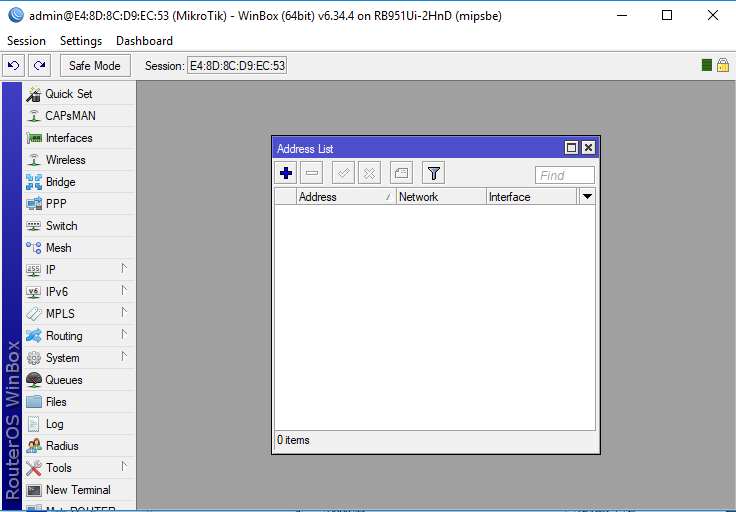
\includegraphics[width=0.8\linewidth]{image2.png}
        \end{center}
        \begin{itemize}
            \item Klik menu IP → Addresses, maka akan muncul kotak windows Address List dan pastikan pada kotak tersebut masih kosong.
        \end{itemize}

    \item \textbf{Setting DHCP Client pada Ether1\\}
        \begin{center}
            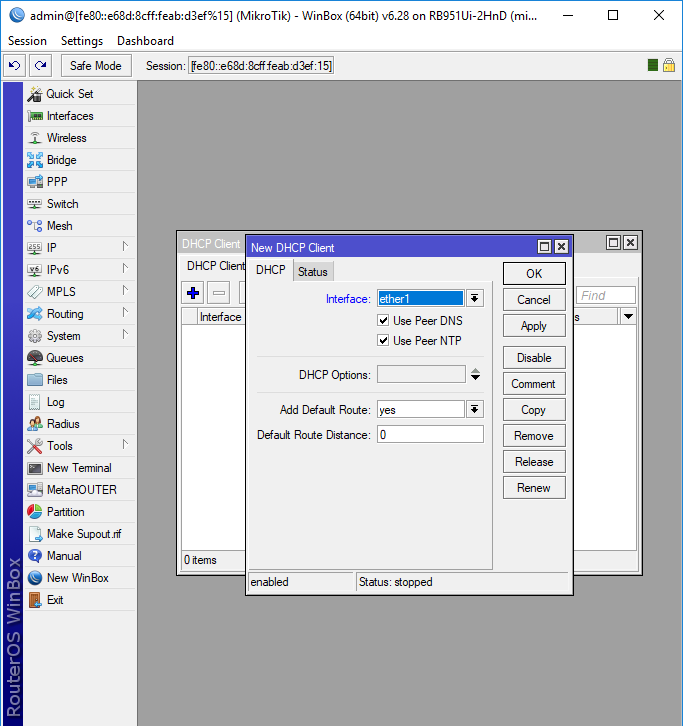
\includegraphics[scale=0.5]{image3.png}
        \end{center}
        \begin{itemize}
            \item Klik menu \textbf{IP $\rightarrow$ DCHP Client}
            \item Maka kemudian akan muncul kotak window DHCP Client, lalu klik tombol Tombol, maka akan muncul kotak window New DHCP Client.
            \item Pada tab DHCP, pilih Interface-nya: Ether1 (dengan cara klik tombol panah bawah, lalu klik Ether1), lalu klik tombol Apply.
            \item Langkah berikutnya klik tab Status, untuk melihat IP Address, Gateway, DHCP Server, Primary DNS, dll. yang didapat DHCP Client di Ether1 dari DHCP Server yang ada di laboratorium, seperti pada Gambar berikut: (alamat IP Address yang di dapat berbeda-beda)
            \item Lalu klik tombol OK, dan pastikan pada kotak windows DHCP Client terdapat interface Ether1 yang telah di konfigurasi sebagai DHCP Client dan pastikan juga pada kotak windows Address List, Ether1 telah mendapat IP yang sama dengan yang ada pada kotak windows DHCP Client.
            \item Sampai dengan langkah ini, berarti Ether1 telah mendapatkan IP yang disewakan oleh DHCP Server yang berada di laboratorium.
        \end{itemize}

    \item \textbf{Menambahkan IP Address pada Ether5}
        \begin{center}
            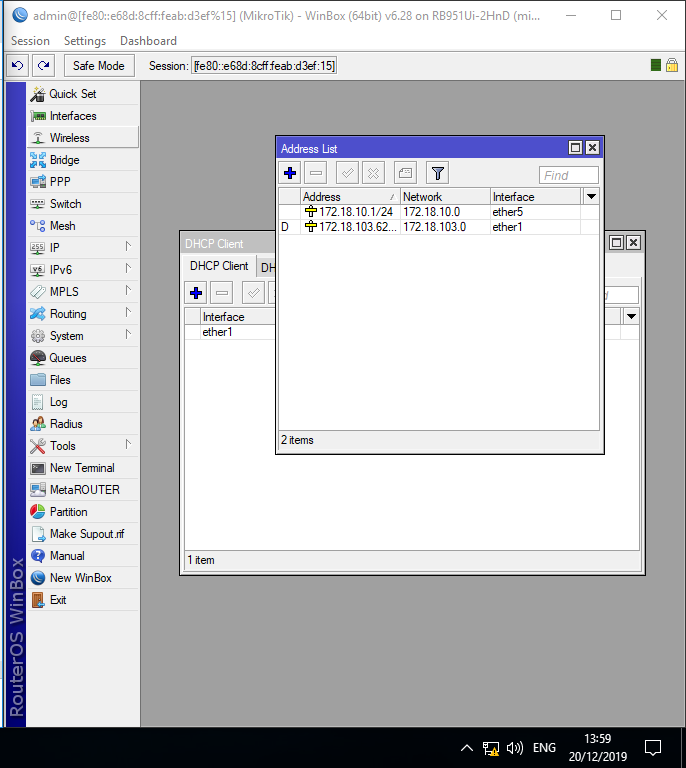
\includegraphics[scale=0.5]{image4.png}
        \end{center}
        \begin{itemize}
            \item Klik menu IP → Addresses, maka akan muncul kotak windows Address List.
            \item Lalu klik tombol , maka akan muncul kotak window New Address. Isikan alamat IP pada pada Address: 172.18.10.1/24 dan Interface: Ether5. Lalu klik Apply (Network, akan terisi secara otomatis)
            \item Klik tombol Apply (Network, akan terisi secara otomatis) seperti pada gambar di bawah ini.
            \item Lalu klik tombol OK, sampai dengan langkah ini, berarti Ether5 memiliki IP yang diisikan dan dapat dilihat pada kotak windows Address List (termasuk Ether1).
        \end{itemize}

    \item \textbf{Setting DHCP Server pada Interface Ether5}
        \begin{center}
            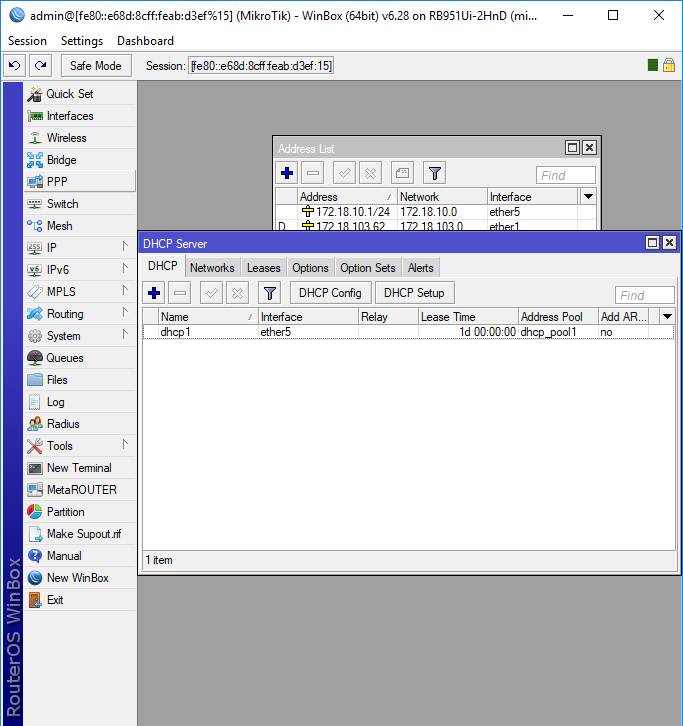
\includegraphics[width=0.8\linewidth]{image5.png}
        \end{center}
        \begin{itemize}
            \item Pilih menu IP → DHCP Server, akan muncul kotak window DHCP Server, lalu klik menu DHCP Setup.
            \item Akan muncul kotak window DHCP Setup, lalu pada isian DHCP Server Interface pilih interface : Ether5 dengan cara klik tombol panah bawah  terlebih dahulu.
            \item Klik tombol Next, pada isian DHCP Address Space alamat network dan netmasknya: 172.18.10.0/24 (secara otomatis berdasarkan setting IP Address pada interface Ether5)
            \item Klik tombol Next, pada isian Gateway for DHCP Network: 172.18.10.1 yang akan dijadikan sebagai gateway untuk setiap DHCP Client-nya (secara otomatis sama dengan IP Address pada interface Ether5).
            \item Klik tombol Next, pada isian Addresses to Give out: 172.18.10.2 – 172.18.10.254 (merupakan range IP Address yang akan diberikan (tepatnya disewakan) ke setiap DHCP Client-nya. (pada praktik kali ini silahkan ubah range-nya dari 172.18.10.2 – 172.18.10.10 sehingga komputer client akan menerima IP Address sesuai range tersebut.
            \item Klik tombol Next, pada isian DNS Server: 172.17.81.253 (akan berisi alamat DNS Server yang telah didapat mikrotik, dapat dilihat pada menu IP → DNS), dapat diganti dengan alamat DNS Server yang lain.
            \item Klik tombol Next, pada isian Lease Time: 3d 00:00:00 (akan berisi lama waktu IP Address dipinjamkan ke Client), isian ini berarti dipinjamkan selama 3 hari. Untuk menghindari penuh atau kehabisan IP, setting Lease-Time jangan terlalu lama, misalkan 1 hari saja.
            \item Klik tombol Next, maka akan tertampil pesan yang menyatakan bahwa setting DHCP telah berhasil.
        \end{itemize}

    \item \textbf{Setting IP address pada komputer (PC 2 dan PC3) yang terhubung ke Ether5 (DHCP Server) melalui Switch.}
        \begin{center}
            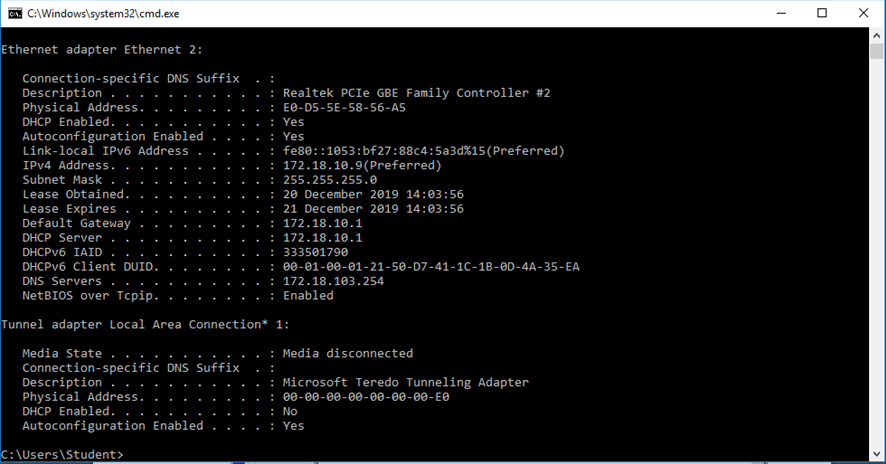
\includegraphics[scale=0.5]{image6.png}
            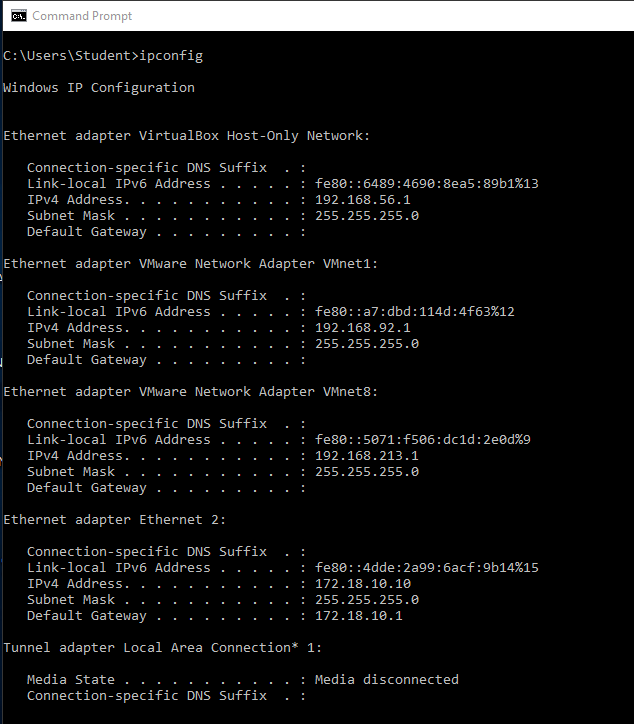
\includegraphics[scale=0.5]{image8.png}
        \end{center}
        \begin{itemize}
            \item Klik kanan pada icon Network , kemudian akan muncul 2 menu dan pilih menu Open Network \& Internet settings.  
            \item Akan muncul kotak window Setting, pilih menu Change adapter option.
            \item Tampil kotak window Network Connections, klik kanan Ethernet (yang mau diberikan IP Address), lalu pilih menu Properties.
            \item Maka akan tampil kotak window Ethernet Properties, double klik Internet Protocol Version 4 (TCP/IPv4), lalu pilih Obtain an IP address automatically dan Obtain DNS server address automatically.
            \item Kemudian klik tombol OK, dan cek IP Address dari komputer tersebut menggunakan aplikasi Comment Prompt dengan perintah ipconfig /all.
            \item Pastikan PC2 dan PC3 keduanya telah mendapatkan IP Address dari DHCP Server dengan range antara 172.18.10.2 - 172.18.10.10.
            \item Lakukan tes koneksi dengan perintah Ping ke Gateway-nya: 172.18.10.1 dan pastikan terkoneksi.
                \begin{center}
                    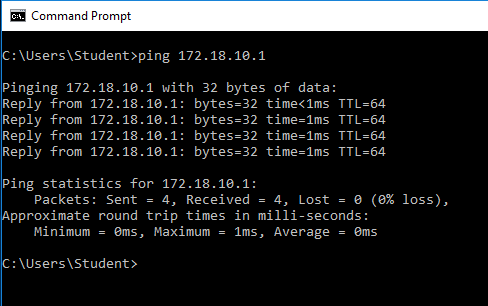
\includegraphics[width=0.8\linewidth]{image9.png}
                \end{center}
        \end{itemize}

    \item \textbf{Cek Koneksi ke Internet Melalui Router Menggunakan Terminal.}
        \begin{center}
            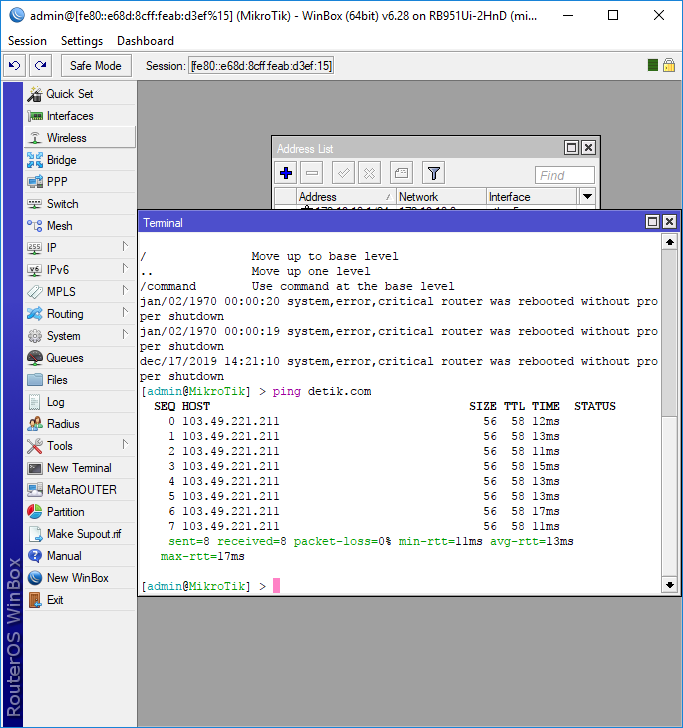
\includegraphics[width=0.8\linewidth]{image10.png}
        \end{center}
        \begin{itemize}
            \item Klik New Terminal, akan muncul kotak window Terminal, berikan perintah untuk cek koneksi ke situs berita: www,detik.com koneksi dengan perintah Ping dan pastikan terkoneksi.
        \end{itemize}

    \item \textbf{Cek Koneksi ke Internet Melalui PC2 dan PC3}
        \begin{center}
            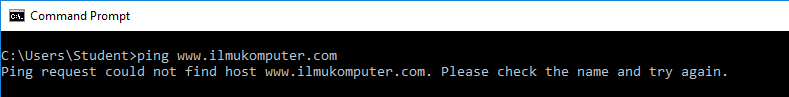
\includegraphics[width=0.8\linewidth]{image11.png}
        \end{center}
        \begin{itemize}
            \item Jalankan aplikasi Command Prompt, berikan perintah untuk cek koneksi ke suatu situs misalnya: www.ilmukomputer.com dengan perintah Ping dan hasilnya akan sama seperti pada gambar berikut yang berarti tidak terkoneksi.
        \end{itemize}

    \item \textbf{Setting Source-Network Address Translation (Src-NAT)}
        \begin{center}
            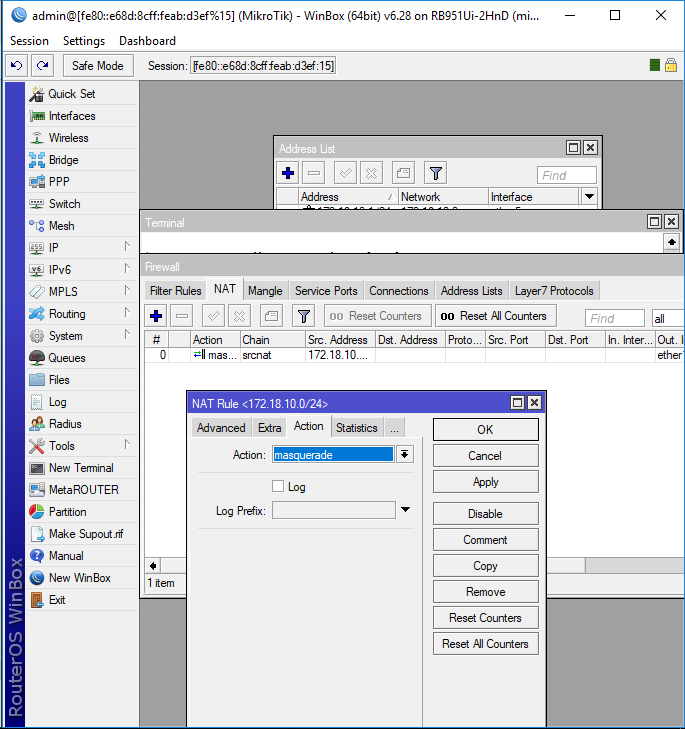
\includegraphics[width=0.8\linewidth]{image12.png}
        \end{center}
        Cek koneksi pada praktik ke-8 membuktikan bahwa router sudah terkoneksi dengan jaringan internet, sedangkan pada praktik ke-9 membuktikan bahwa PC2 dan PC3 yang terhubung ke Ether5 belum terkoneksi dengan jaringan internet. Setting ini akan mengubah source address dari sebuah paket data, yang berasal dari PC yang terhubung ke Ether5 diubah ke source address-nya milik Ether1 yang sudah sudah terbukti dapat terkoneksi dengan internet, sehingga menjadikan PC yang terhubung ke Ether5 dapat terkoneksi dengan jaringan internet.
        \begin{itemize}
            \item Pilih menu IP → Firewall, akan muncul kotak window Firewall, lalu klik tab NAT.
            \item Kemudian klik tombol  , maka akan muncul kotak window New NAT Rule, klik tab General dan lakukan pengisian pada Chain: srcnat (untuk mengubah source address dari sebuah paket data), Src. Address: 172.18.10.0/24 (source address yang diubah memiliki alamat network 172.18.10.0 dan netmask: 255.255.255.0) dan Out. Interface:Ether1 (interface yang akan dikenali dari luar).
            \item Klik tab Action, pada isian Action:masquerade (ini berarti bahwa source address 172.18.10.0/24 ditopengkan sehingga nanti akan dikenal dengan source addres-nya Ether1, yaitu: 172.17.25.111/24, kemudian klik tombol Apply.
            \item Kemudian klik tombol OK, yang berarti setting Src-NAT telah selesai.
        \end{itemize}

    \item \textbf{Cek Kembali Koneksi ke Internet Melalui PC2 dan PC3 yang terhubung ke Ether6.}
        \begin{itemize}
            \item Jalankan aplikasi Command Prompt, berikan perintah untuk cek koneksi ke situs berita: www.ilmukomputer.com koneksi dengan perintah Ping dan hasilnya akan berbeda seperti pada gambar berikut.
                \begin{center}
                    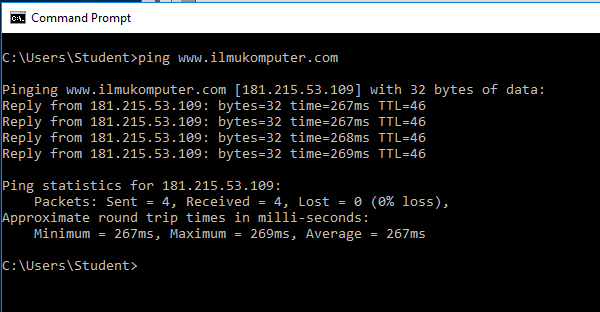
\includegraphics[width=0.8\linewidth]{image14.png}
                \end{center}
        \end{itemize}

    \item \textbf{Membuat Firewall untuk Memblock Akses Internet dari PC2 dengan IP Address.}
        \begin{center}
            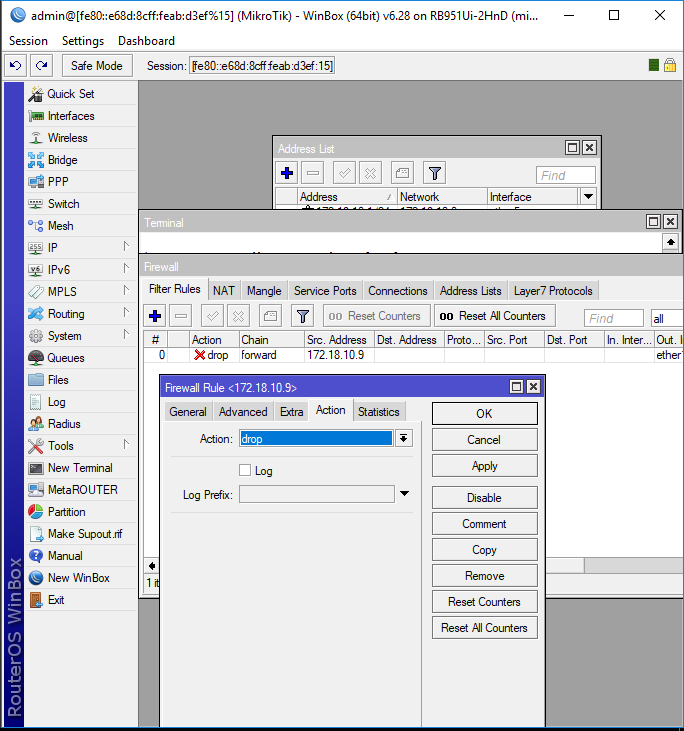
\includegraphics[width=0.8\linewidth]{image15.png}
        \end{center}
        \begin{itemize}
            \item Pilih menu IP → Firewall, akan muncul kotak window Firewall, lalu klik tab Filter Rules.
            \item Kemudian klik tombol , maka akan muncul kotak window New Firewall Rule, klik tab General dan lakukan pengisian pada Chain: forward (untuk memproses trafik paket data yang hanya melewati router), Src. Address: 172.18.10.10 (source address-nya PC2 yang akan di blok) dan Out. Interface:Ether1.
            \item Klik tab Action dan lakukan pengisian pada Chain: drop (yang berarti packet data dari PC2 dengan IP Address 172.18.10.10, jika keluar melalui interface Ether1 akan di drop).
        \end{itemize}

    \item \textbf{Cek Akses Internet dari PC2 dan PC3.}
        \begin{center}
            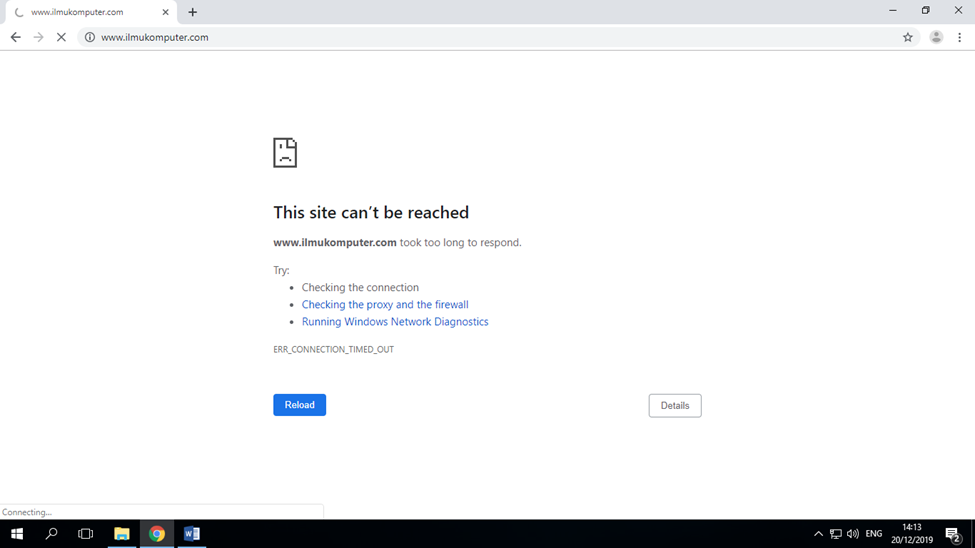
\includegraphics[width=0.8\linewidth]{image16.png}
        \end{center}
        \begin{itemize}
            \item Jalankan web browser, kemudian buka situs www.ilmukomputer.com atau situs lain, jika tidak dapat akses situs tersebut berarti konfigurasi sudah benar.
        \end{itemize}

    \item \textbf{Membuat Firewall untuk Memblock Akses Internet dari PC2 ke suatu situs.}
        \begin{center}
            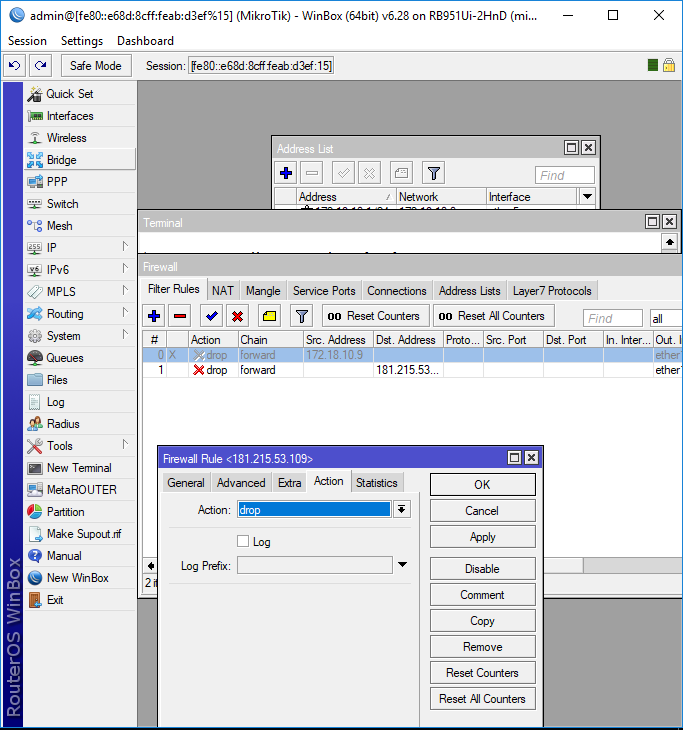
\includegraphics[width=0.8\linewidth]{image17.png}
        \end{center}
        \begin{itemize}
            \item Pilih menu IP → Firewall, akan muncul kotak window Firewall, lalu klik tab Filter Rules.
            \item Pilih hasil konfigurasi “Membuat firewall untuk memblock akses internet dari PC2 dengan IP Address” sebelumnya, lalu klik tombol Disable, untuk mengembalikan agar PC2 dapat akses internet lagi.
            \item Pastikan PC2 dapat akses internet (silahkan akses situs www.ilmukomputer.com dan pastikan berhasil).
            \item Cek koneksi ke situs www.ilmukomputer.com, menggunakan Command Prompt dengan perintah ping www,ilmukomputer.com dan catat IP Address-nya.
            \item Kemudian klik tombol  , maka akan muncul kotak window New Firewall Rule, klik tab General dan lakukan pengisian pada Chain: forward (untuk memproses trafik paket data yang hanya melewati router), Dst. Address: 181.215.53.109 (destination address: IP Address-nya situs www.ilmukomputer.com) dan Out. Interface:Ether1.
            \item Klik tab Action dan lakukan pengisian pada Chain: drop (yang berarti akses ke situs www.ilmukomputer.com dengan IP Address: 181.215.53.109 akan di drop, sedangkan ke situs lain masih dapat diakses).
        \end{itemize}

    \item \textbf{Cek akses Internet dari PC2 dan PC3.}
        \begin{figure}[]
            \centering
            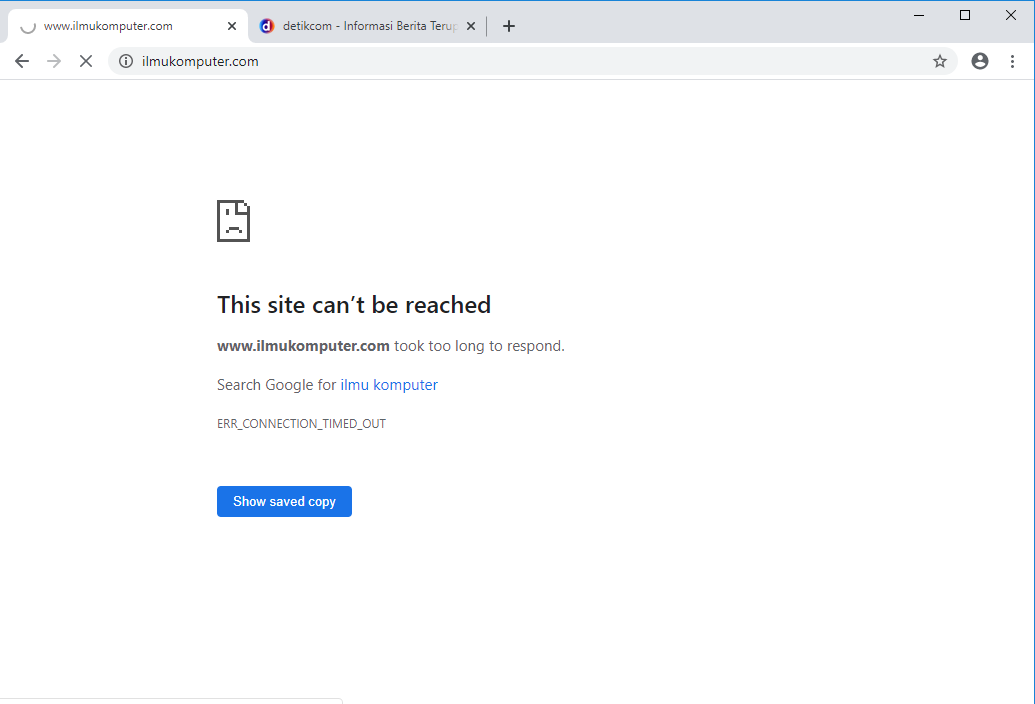
\includegraphics[width=0.8\linewidth]{image18.png}
            \caption*{PC 2}
            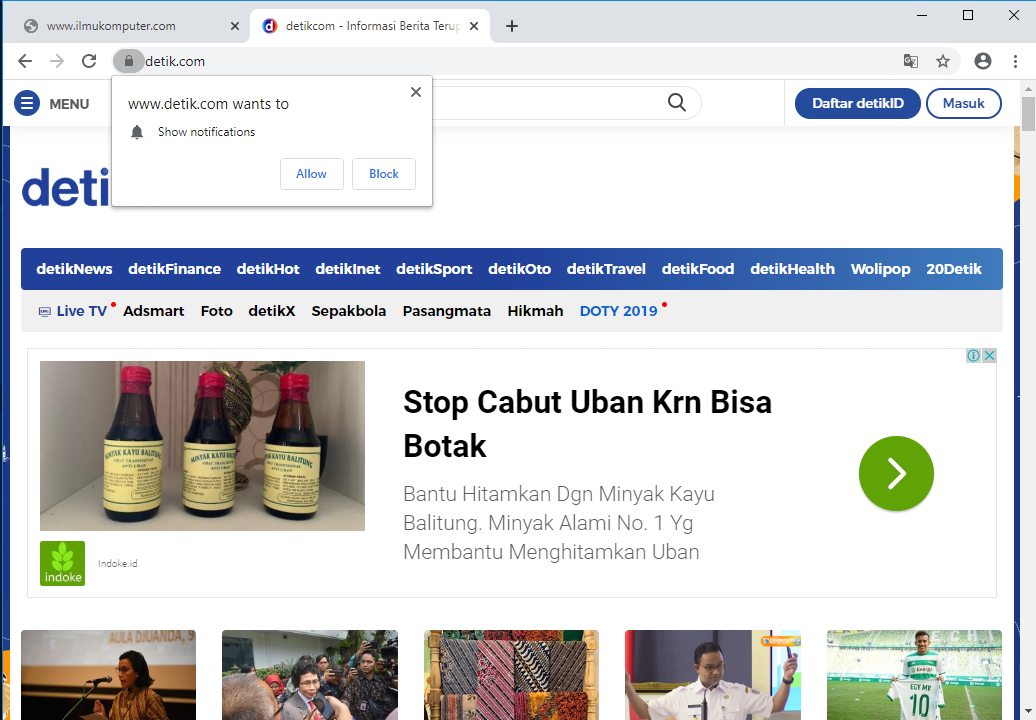
\includegraphics[width=0.8\linewidth]{image19.png}
            \caption*{PC 3}
        \end{figure}

\end{enumerate}

\section{Latihan}
\begin{enumerate}
    \item Konfigurasi Mikrotik agar PC2 tidak dapat akses internet menggunakan MAC Address.
        \begin{center}
            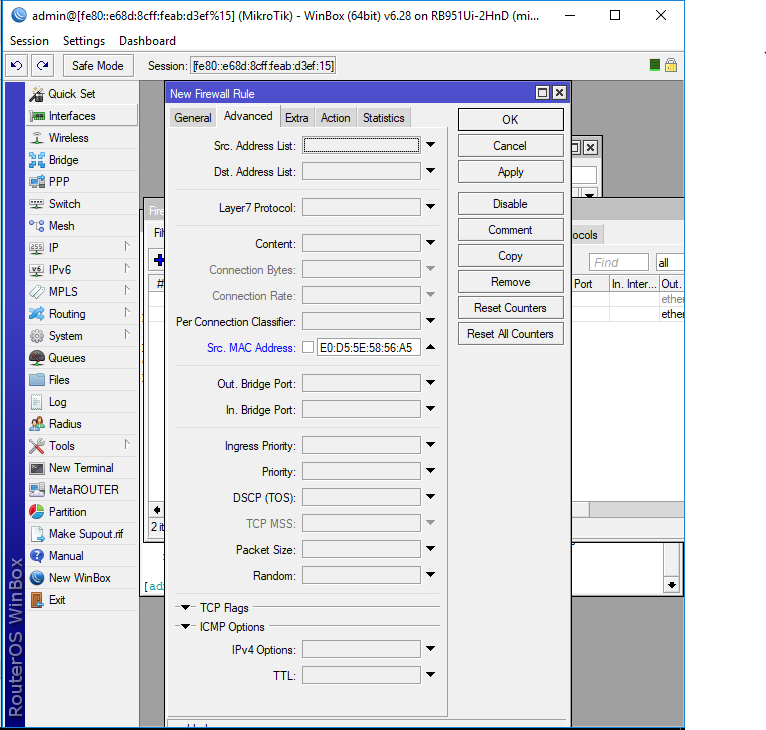
\includegraphics[width=0.8\linewidth]{image20.png}
        \end{center}
        \begin{itemize}
            \item Pilih menu IP → Firewall, akan muncul kotak window Firewall, lalu klik tab Filter Rules.
            \item Kemudian klik tombol , maka akan muncul kotak window New Firewall Rule, klik tab Advanced dan lakukan pengisian pada Src. MAC Address: E0:D5:5E:58:56:A5 (MAC address-nya PC2 yang akan di blok).
            \item Tampilan setalah melakukan blok firewall untuk PC 2 agar tidak dapat mengakses internet
                \begin{center}
                    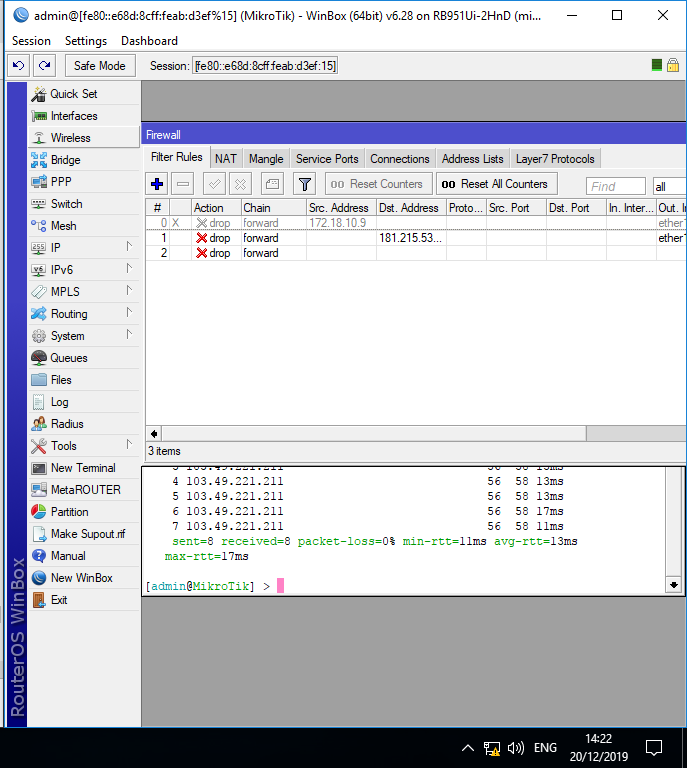
\includegraphics[width=0.8\linewidth]{image21.png}
                \end{center}
        \end{itemize}

    \item Konfigurasi Mikrotik agar PC2 dapat akses situs www.ilmukomputer.com, sedangkan PC3 tidak dapat akses situs www.ilmukomputer.com
        \begin{itemize}
            \item Pilih menu IP → Firewall, akan muncul kotak window Firewall, lalu klik tab Filter Rules.
            \item Pilih hasil konfigurasi “Membuat firewall untuk memblock akses internet dari PC2 dengan MAC Address” sebelumnya, lalu klik tombol Disable, untuk mengembalikan agar PC2 dapat akses internet lagi.
            \item Pastikan PC2 dapat akses internet (silahkan akses situs www.ilmukomputer.com dan pastikan berhasil).
            \item Cek koneksi ke situs www.ilmukomputer.com, menggunakan Command Prompt dengan perintah ping www,ilmukomputer.com dan catat IP Address-nya.
            \item Kemudian klik tombol  , maka akan muncul kotak window New Firewall Rule, klik tab General dan lakukan pengisian pada Chain: forward (untuk memproses trafik paket data yang hanya melewati router), Dst. Address: 181.215.53.109 (destination address: IP Address-nya situs www.ilmukomputer.com) dan Src. Address: 172.18.10.10
                \begin{center}
                    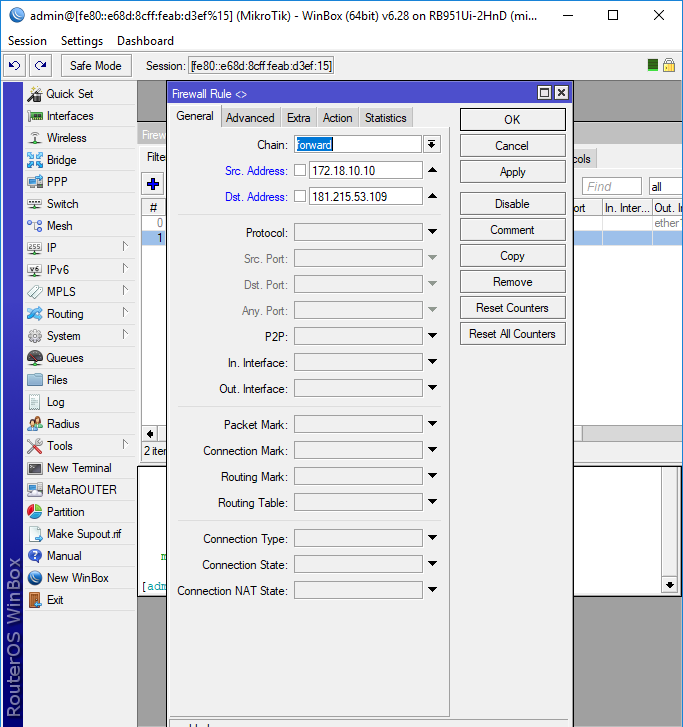
\includegraphics[width=0.8\linewidth]{image23.png}
                \end{center}
            \item Klik tab Action dan lakukan pengisian pada Chain: drop (yang berarti akses ke situs ilmukomputer.com dengan IP Address: 181.215.53.109 akan di drop, sedangkan ke situs lain masih dapat diakses).
                \begin{center}
                    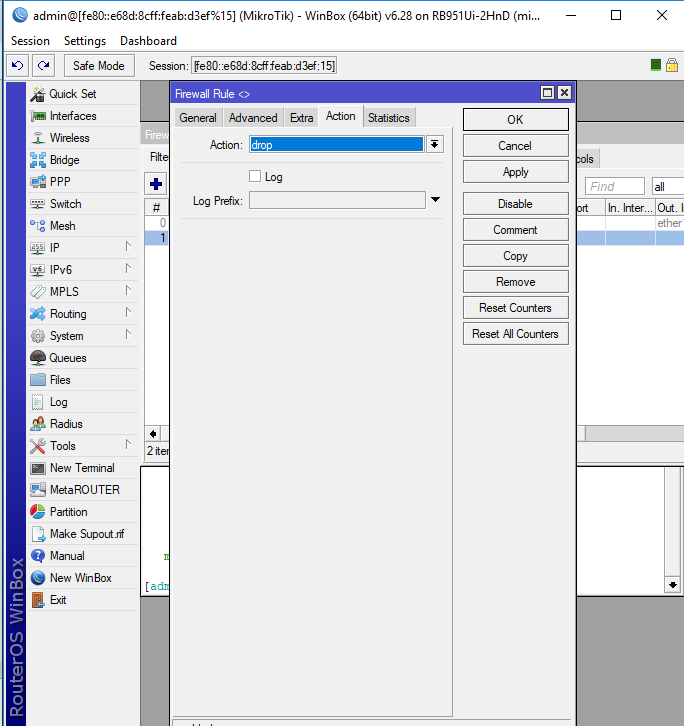
\includegraphics[width=0.8\linewidth]{image24.png}
                \end{center}
            \item Setelah itu kita lakukan tes koneksi dari PC3 setelah dilakukan konfigruasi mikrotik agar PC 3 tidak dapat mengakses situs www.ilmukomputer.com
                 \begin{center}
                    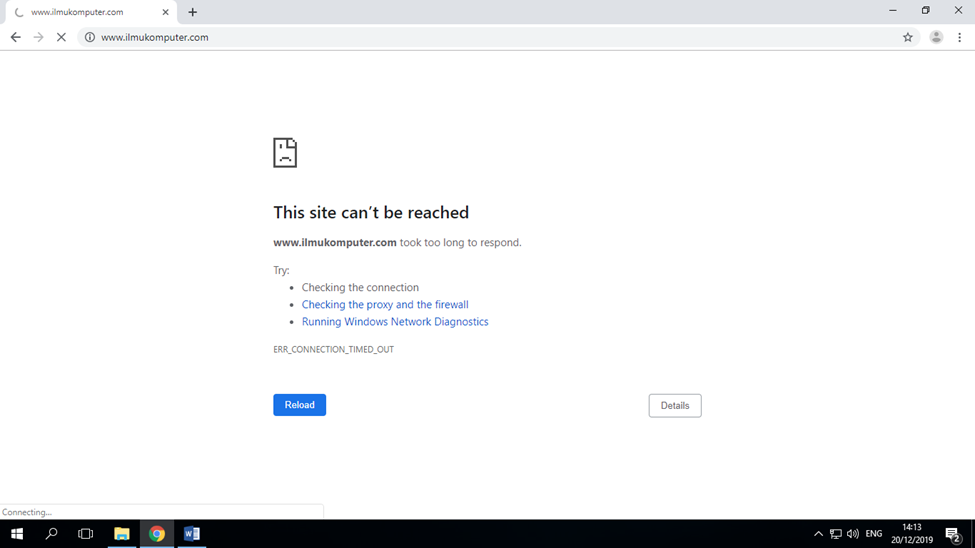
\includegraphics[width=0.8\linewidth]{image16.png}
                \end{center}
       \end{itemize}

\end{enumerate}

\newpage

\section{Tugas}
\paragraph{}
Sebutkan kegunaan yang lain dari pembuatan Firewall selain yang telah dipraktikkan
\begin{itemize}
    \item Filter Rules\\
    Filter rule biasanya digunakan untuk melakukan kebijakan boleh atau tidaknya sebuah trafik ada dalam jaringan, identik dengan accept atau drop. Pada menu Firewall → Filter Rules terdapat 3 macam chain yang tersedia. Chain tersebut antara lain adalah Forward, Input, Output.

    \item NAT (Network Address Translation)\\
    Pada menu Firewall → NAT terdapat 2 macam opsi chain yang tersedia, yaitu dst-nat dan src-nat. Dan fungsi dari NAT sendiri adalah untuk melakukan pengubahan Source Address maupun Destination Address.

    \item Mangle\\
    Pada menu Firewall → Mangle terdapat 4 macam pilihan untuk chain, yaitu Forward, Input, Output, Prerouting, dan Postrouting. Mangle sendiri memiliki fungsi untuk menandai sebuah koneksi atau paket data, yang melewati route, masuk ke router, ataupun yang keluar dari router. Pada implementasinya Mangle sering dikombinasikan dengan fitur lain seperti Management Bandwith, Routing policy, dll.
\end{itemize}

\section{Kesimpulan}
\paragraph{}
Mahasiswa mampu melakukan konfigurasi pada Router untuk memblok akses internet menggunakan Firewall.
\end{document}
